% =============================================================================
% Long-Range Dependence as Informative Features for Machine Learning
% in Financial Forecasting
% =============================================================================
% Authors: Akash Deep, Nicholas Appiah
% Advisor: Dr. Svetlozar Rachev
% Texas Tech University
% January 2025
% =============================================================================

\documentclass[12pt,a4paper]{article}

% Packages
\usepackage[utf8]{inputenc}
\usepackage[T1]{fontenc}
\usepackage{amsmath,amssymb,amsfonts}
\usepackage{graphicx}
\usepackage{booktabs}
\usepackage{multirow}
\usepackage{array}
\usepackage{caption}
\usepackage{subcaption}
\usepackage{natbib}
\usepackage{hyperref}
\usepackage{geometry}
\usepackage{setspace}
\usepackage{threeparttable}
\usepackage{float}

\geometry{margin=1in}
\onehalfspacing

% Figure path - all figures in src folder
\graphicspath{{src/}}

% Custom commands
\newcommand{\RV}{\text{RV}}
\newcommand{\VIX}{\text{VIX}}
\newcommand{\MSE}{\text{MSE}}
\newcommand{\MAE}{\text{MAE}}
\newcommand{\QLIKE}{\text{QLIKE}}

\title{\textbf{Long-Range Dependence as Informative Features for Machine Learning in Financial Forecasting}}

\author{
Akash Deep\thanks{Department of Mathematics and Statistics, Texas Tech University. Email: akash.deep@ttu.edu} \and
Nicholas Appiah\thanks{Department of Mathematics and Statistics, Texas Tech University.}
}

\date{January 2025}

\begin{document}

\maketitle

% =============================================================================
% ABSTRACT
% =============================================================================
\begin{abstract}
We investigate whether estimated parameters from Long-Range Dependence (LRD) models contain predictive information for volatility forecasting beyond their traditional role in stationarity transformation. Using a sample of 125 S\&P 500 stocks over 25 years (2000--2025), we construct novel features from rolling estimates of the memory parameter $\hat{d}$, including memory dynamics ($\Delta\hat{d}$, Vol($\hat{d}$)) and cross-sectional memory dispersion. Our hybrid HAR-LRD model, which augments the standard HAR-RV benchmark with LRD features, achieves consistent forecast improvements across 90\% of stocks with an average MSE reduction of 3.4\%. Feature importance analysis reveals that cross-sectional mean memory is the second most important predictor, accounting for 37\% of total feature importance when combined with other LRD measures. Robustness analysis shows that LRD features are particularly valuable during high-volatility regimes, with improvements of 4.9\% during the COVID period and 2.7\% during the 2008 Financial Crisis. These findings support treating memory parameters as informative features rather than mere nuisance parameters.
\end{abstract}

\noindent\textbf{Keywords:} Long-range dependence, volatility forecasting, machine learning, memory parameter, HAR-RV, feature engineering

\noindent\textbf{JEL Classification:} C22, C45, C53, G17

\newpage
\tableofcontents
\newpage

% =============================================================================
% 1. INTRODUCTION
% =============================================================================
\section{Introduction}
\label{sec:introduction}

Long-range dependence (LRD) in financial time series, particularly in volatility, has been extensively documented since the seminal work of \citet{ding1993long}. The fractional differencing parameter $d$ characterizes the rate of decay in autocorrelations and has profound implications for forecasting, risk management, and derivative pricing. However, the traditional approach treats the estimated memory parameter $\hat{d}$ primarily as a tool for achieving stationarity through fractional differencing, discarding potentially
valuable information contained in the estimate itself.

\vspace{0.3cm}
\noindent
Empirical evidence shows that long memory is primarily a feature of volatility rather than returns and persists across markets and sampling frequencies
\citep{he2025lrd, baillie2019longmemory}. Fractionally integrated models such as ARFIMA and FIGARCH provide a natural framework for capturing this behavior and remain statistically significant even after accounting for heavy-tailed innovations and nonlinear dynamics \citep{he2025lrd}. These findings suggest that the long-memory parameter summarizes fundamental aspects of volatility persistence.

\vspace{0.3cm}
\noindent
In parallel, reduced form approaches such as the Heterogeneous Autoregressive (HAR) model have been shown to approximate long-memory behavior using multi-scale volatility
aggregation. While HAR models perform competitively in practice, recent evidence indicates that volatility dynamics and HAR coefficients vary across market regimes, particularly during periods of heightened uncertainty \citep{blake2025regime}. This instability highlights the importance of modeling time variation in persistence.

\vspace{0.3cm}
\noindent
At the same time, machine learning methods have gained prominence in volatility forecasting. Recent studies demonstrate that tree-based and ensemble learning methods outperform traditional econometric benchmarks when supplied with rich feature sets
\citep{omer2026mlrv, zhang2024intraday}. These gains are especially pronounced at longer forecast horizons, where persistence and long-memory effects dominate volatility dynamics.

\vspace{0.3cm}
\noindent
Despite these advances, existing approaches typically learn long-range dependence
implicitly through lagged inputs or model structure. The estimated memory parameter itself is rarely incorporated explicitly into the forecasting stage. This omission is notable given evidence that volatility regimes, structural changes, and higher-order dependence play a central role in predictive performance \citep{blake2025regime}.

\vspace{0.3cm}
\noindent
Recent regime-aware and feature-engineered forecasting frameworks further demonstrate that explicitly incorporating structural information improves volatility prediction,
particularly during turbulent periods \citep{blake2025regime}. These findings motivate a forecasting strategy that conditions directly on descriptors of volatility persistence.

\vspace{0.3cm}
\noindent
This paper proposes a novel perspective: we treat $\hat{d}$ and related statistics as
\emph{informative features} for machine learning algorithms rather than mere nuisance
parameters. Our key insight is that the memory parameter captures fundamental properties of the underlying price process that may have predictive power for future volatility, independent of its role in model specification.

\subsection{Research Questions}

We address the following research questions:
\begin{enumerate}
    \item Does the estimated fractional differencing parameter $\hat{d}$ contain predictive information for volatility beyond its role in stationarity transformation?
    \item Can machine learning exploit time-variation in long-memory parameters to improve forecasting during regime changes?
    \item What is the relative importance of LRD-based features compared to traditional HAR components?
\end{enumerate}

\subsection{Main Contributions}

Our main contributions are:
\begin{enumerate}
    \item We systematically document the cross-sectional and time-series properties of memory parameter estimates across 125 stocks over 25 years.
    \item We construct novel feature vectors from LRD estimation, including memory dynamics ($\Delta\hat{d}$, Vol($\hat{d}$), Trend($\hat{d}$)) and cross-sectional memory dispersion.
    \item We demonstrate that augmenting standard HAR-RV models with LRD features yields consistent forecast improvements.
    \item We show that cross-sectional memory dispersion has substantial predictive power, ranking as the second most important feature in our analysis.
    \item We document that LRD features are most valuable during high-volatility regimes, providing important insights for risk management.
\end{enumerate}

% =============================================================================
% 2. METHODOLOGY
% =============================================================================
\section{Methodology}
\label{sec:methodology}

\subsection{Long-Range Dependence and Memory Parameter Estimation}

A covariance stationary process $\{X_t\}$ exhibits long-range dependence if its autocorrelation function $\rho(k)$ decays hyperbolically:
\begin{equation}
    \rho(k) \sim c_\rho k^{2d-1} \quad \text{as } k \to \infty
\end{equation}
where $d \in (0, 0.5)$ is the memory parameter. For $d > 0$, autocorrelations are non-summable, indicating persistent dependence structures that standard ARMA models cannot capture.

\subsubsection{GPH Estimator}

The Geweke-Porter-Hudak (GPH) log-periodogram estimator \citep{geweke1983estimation} exploits the relationship between the spectral density and the memory parameter near the origin:
\begin{equation}
    f(\lambda) \sim c_f \lambda^{-2d} \quad \text{as } \lambda \to 0^+
\end{equation}

Taking logarithms of the periodogram ordinates at Fourier frequencies $\lambda_j = 2\pi j/T$ yields the regression:
\begin{equation}
    \ln I(\lambda_j) = c - 2d \ln \lambda_j + \epsilon_j, \quad j = 1, \ldots, m
\end{equation}

The GPH estimator is:
\begin{equation}
    \hat{d}_{\text{GPH}} = -\frac{1}{2} \frac{\sum_{j=1}^m (x_j - \bar{x})(\ln I(\lambda_j) - \overline{\ln I})}{\sum_{j=1}^m (x_j - \bar{x})^2}
\end{equation}
where $x_j = \ln \lambda_j$ and $m = \lfloor T^{0.5} \rfloor$ is the bandwidth parameter. The standard error is $\text{SE}(\hat{d}) = \frac{\pi}{\sqrt{24m}}$.

\subsubsection{Local Whittle Estimator}

The Local Whittle estimator \citep{robinson1995gaussian} minimizes the local Whittle objective function:
\begin{equation}
    Q(d) = \frac{1}{m}\sum_{j=1}^m \left[\ln(\lambda_j^{-2d} \hat{G}) + \frac{I(\lambda_j)}{\lambda_j^{-2d}\hat{G}}\right]
\end{equation}
where $\hat{G}(d) = \frac{1}{m}\sum_{j=1}^m \lambda_j^{2d} I(\lambda_j)$. This estimator is asymptotically more efficient than GPH:
\begin{equation}
    \hat{d}_{\text{LW}} = \arg\min_d Q(d), \quad \text{SE}(\hat{d}) = \frac{1}{2\sqrt{m}}
\end{equation}

\subsubsection{FIGARCH Model}

As a parametric complement to our semi-parametric estimators, we also employ the Fractionally Integrated GARCH (FIGARCH) model of \citet{baillie1996figarch}. The FIGARCH(1,$d$,1) specification models the conditional variance as:
\begin{equation}
    \sigma_t^2 = \omega + \beta \sigma_{t-1}^2 + \left[1 - \beta L - (1-\phi L)(1-L)^d\right] \epsilon_t^2
\end{equation}
where $L$ is the lag operator, $d \in (0, 1)$ is the fractional integration parameter, and $(1-L)^d$ is the fractional differencing operator defined via the binomial expansion:
\begin{equation}
    (1-L)^d = \sum_{k=0}^{\infty} \binom{d}{k} (-L)^k = 1 - dL - \frac{d(1-d)}{2}L^2 - \cdots
\end{equation}

For $d \in (0, 0.5)$, the process exhibits stationary long memory with hyperbolic decay in the autocorrelation of squared returns. When $d = 0$, FIGARCH reduces to standard GARCH(1,1). The FIGARCH model provides a parametric validation of our semi-parametric LRD estimates and allows for direct comparison of memory parameter estimates across methodologies.

\subsection{Feature Engineering from LRD Estimates}

We construct a comprehensive feature vector $\mathbf{F}_t^{\text{LRD}}$ from rolling window estimates of the memory parameter:

\begin{equation}
    \mathbf{F}_t^{\text{LRD}} = \begin{pmatrix}
        \hat{d}_t \\
        \text{SE}(\hat{d}_t) \\
        \Delta\hat{d}_t \\
        \text{Vol}(\hat{d})_t \\
        \text{Trend}(\hat{d})_t \\
        \bar{d}_t^{\text{CS}} \\
        \sigma_d^{\text{CS}}
    \end{pmatrix}
\end{equation}

where:
\begin{itemize}
    \item $\hat{d}_t$: Rolling 500-day GPH estimate of memory parameter
    \item $\text{SE}(\hat{d}_t)$: Standard error of the estimate
    \item $\Delta\hat{d}_t = \hat{d}_t - \hat{d}_{t-1}$: First difference (memory dynamics)
    \item $\text{Vol}(\hat{d})_t = \sqrt{\frac{1}{20}\sum_{i=0}^{19}(\hat{d}_{t-i} - \bar{d})^2}$: Rolling volatility of $\hat{d}$
    \item $\text{Trend}(\hat{d})_t$: 22-day linear trend coefficient
    \item $\bar{d}_t^{\text{CS}} = \frac{1}{N}\sum_{i=1}^N \hat{d}_{i,t}$: Cross-sectional mean memory
    \item $\sigma_d^{\text{CS}} = \sqrt{\frac{1}{N}\sum_{i=1}^N (\hat{d}_{i,t} - \bar{d}_t^{\text{CS}})^2}$: Cross-sectional dispersion
\end{itemize}

\subsection{Benchmark Model: HAR-RV}

The Heterogeneous Autoregressive model of Realized Volatility (HAR-RV) by \citet{corsi2009simple} serves as our benchmark:
\begin{equation}
    \RV_{t+1} = \alpha + \beta_d \RV_t^{(d)} + \beta_w \RV_t^{(w)} + \beta_m \RV_t^{(m)} + \varepsilon_{t+1}
\end{equation}
where:
\begin{align}
    \RV_t^{(d)} &= \RV_t & \text{(daily)} \\
    \RV_t^{(w)} &= \frac{1}{5}\sum_{i=0}^{4} \RV_{t-i} & \text{(weekly average)} \\
    \RV_t^{(m)} &= \frac{1}{22}\sum_{i=0}^{21} \RV_{t-i} & \text{(monthly average)}
\end{align}

In the absence of high-frequency data, we use squared returns as a volatility proxy: $\RV_t \approx r_t^2$.

\subsection{Hybrid LRD-ML Models}

\subsubsection{HAR-LRD: Linear Extension}

We extend HAR-RV by including LRD features:
\begin{equation}
    \RV_{t+1} = \alpha + \beta_d \RV_t^{(d)} + \beta_w \RV_t^{(w)} + \beta_m \RV_t^{(m)} + \gamma' \mathbf{F}_t^{\text{LRD}} + \varepsilon_{t+1}
\end{equation}

\subsubsection{XGBoost-LRD: Nonlinear Extension}

For nonlinear interactions, we employ XGBoost \citep{chen2016xgboost} with the combined feature set:
\begin{equation}
    \mathbf{X}_t = [\RV_t^{(d)}, \RV_t^{(w)}, \RV_t^{(m)}, \mathbf{F}_t^{\text{LRD}}, \VIX_t]
\end{equation}

\subsection{Forecast Evaluation}

\subsubsection{Loss Functions}

We evaluate forecasts using Mean Squared Error:
\begin{equation}
    \MSE = \frac{1}{T}\sum_{t=1}^T (\sigma_t^2 - \hat{\sigma}_t^2)^2
\end{equation}

\subsubsection{Diebold-Mariano Test}

For pairwise model comparison, we use the Diebold-Mariano test \citep{diebold1995comparing}:
\begin{equation}
    \text{DM} = \frac{\bar{d}}{\sqrt{\hat{V}(\bar{d})/T}} \xrightarrow{d} N(0,1)
\end{equation}
where $d_t = L(e_{1t}) - L(e_{2t})$ is the loss differential and $\hat{V}(\bar{d})$ is the HAC variance estimator.

% =============================================================================
% 3. DATA
% =============================================================================
\section{Data}
\label{sec:data}

\subsection{Sample Construction}

Our sample consists of 125 stocks from the S\&P 500 index with at least 70\% data coverage over the period January 2000 to January 2025 (6,296 trading days). Daily closing prices are obtained from Yahoo Finance and Bloomberg. We compute log returns and winsorize at the 0.1\% and 99.9\% percentiles to mitigate the impact of stock splits and data errors.

\subsection{Summary Statistics}

Table \ref{tab:summary_stats} presents summary statistics for daily returns across our sample.

\begin{table}[H]
\centering
\caption{Summary Statistics for Daily Stock Returns}
\label{tab:summary_stats}
\small
\begin{tabular}{lcccccc}
\toprule
 & Mean & Std & Skewness & Kurtosis & Min & Max \\
 & (\% ann.) & (\% ann.) & & & (\%) & (\%) \\
\midrule
\multicolumn{7}{l}{\textbf{Panel A: Pooled Sample}} \\
All Stocks (N=125) & 9.67 & 32.47 & -0.05 & 7.98 & -13.29 & 13.19 \\
\midrule
\multicolumn{7}{l}{\textbf{Panel B: By Sector}} \\
Communication (n=6) & 9.82 & 33.33 & 0.03 & 6.09 & -13.17 & 13.19 \\
Consumer Disc. (n=11) & 11.21 & 34.28 & 0.02 & 6.13 & -13.29 & 13.19 \\
Consumer Staples (n=12) & 8.00 & 22.83 & -0.20 & 9.87 & -12.53 & 12.35 \\
Energy (n=9) & 9.31 & 36.16 & -0.12 & 5.45 & -13.29 & 13.19 \\
Financials (n=13) & 6.77 & 36.70 & 0.01 & 7.33 & -13.29 & 13.19 \\
Healthcare (n=12) & 9.67 & 27.38 & -0.11 & 7.13 & -12.88 & 12.60 \\
Industrials (n=13) & 9.96 & 29.23 & -0.13 & 6.44 & -13.16 & 13.12 \\
Materials (n=11) & 9.69 & 32.96 & -0.08 & 5.56 & -13.21 & 13.19 \\
Real Estate (n=12) & 11.23 & 33.62 & -0.06 & 9.70 & -13.29 & 13.19 \\
Technology (n=12) & 11.12 & 38.73 & -0.05 & 5.28 & -13.21 & 13.02 \\
Utilities (n=12) & 9.45 & 22.93 & -0.21 & 10.64 & -13.10 & 13.11 \\
\bottomrule
\end{tabular}
\begin{tablenotes}\small
\item \textit{Notes:} Sample period: January 2000 to January 2025 (6,296 trading days). Mean and Std are annualized. Returns are log returns, winsorized at 0.1\% and 99.9\%.
\end{tablenotes}
\end{table}
\noindent
The pooled sample exhibits typical stylized facts: near-zero mean, moderate volatility (32.47\% annualized), negative skewness, and substantial excess kurtosis (7.98), confirming fat tails. Technology and Financials show highest volatility, while Consumer Staples and Utilities are most stable.

\newpage
\subsection{Evidence of Long-Range Dependence}

Figure \ref{fig:data_overview} illustrates the key stylized facts motivating our analysis.

\begin{figure}[H]
    \centering
    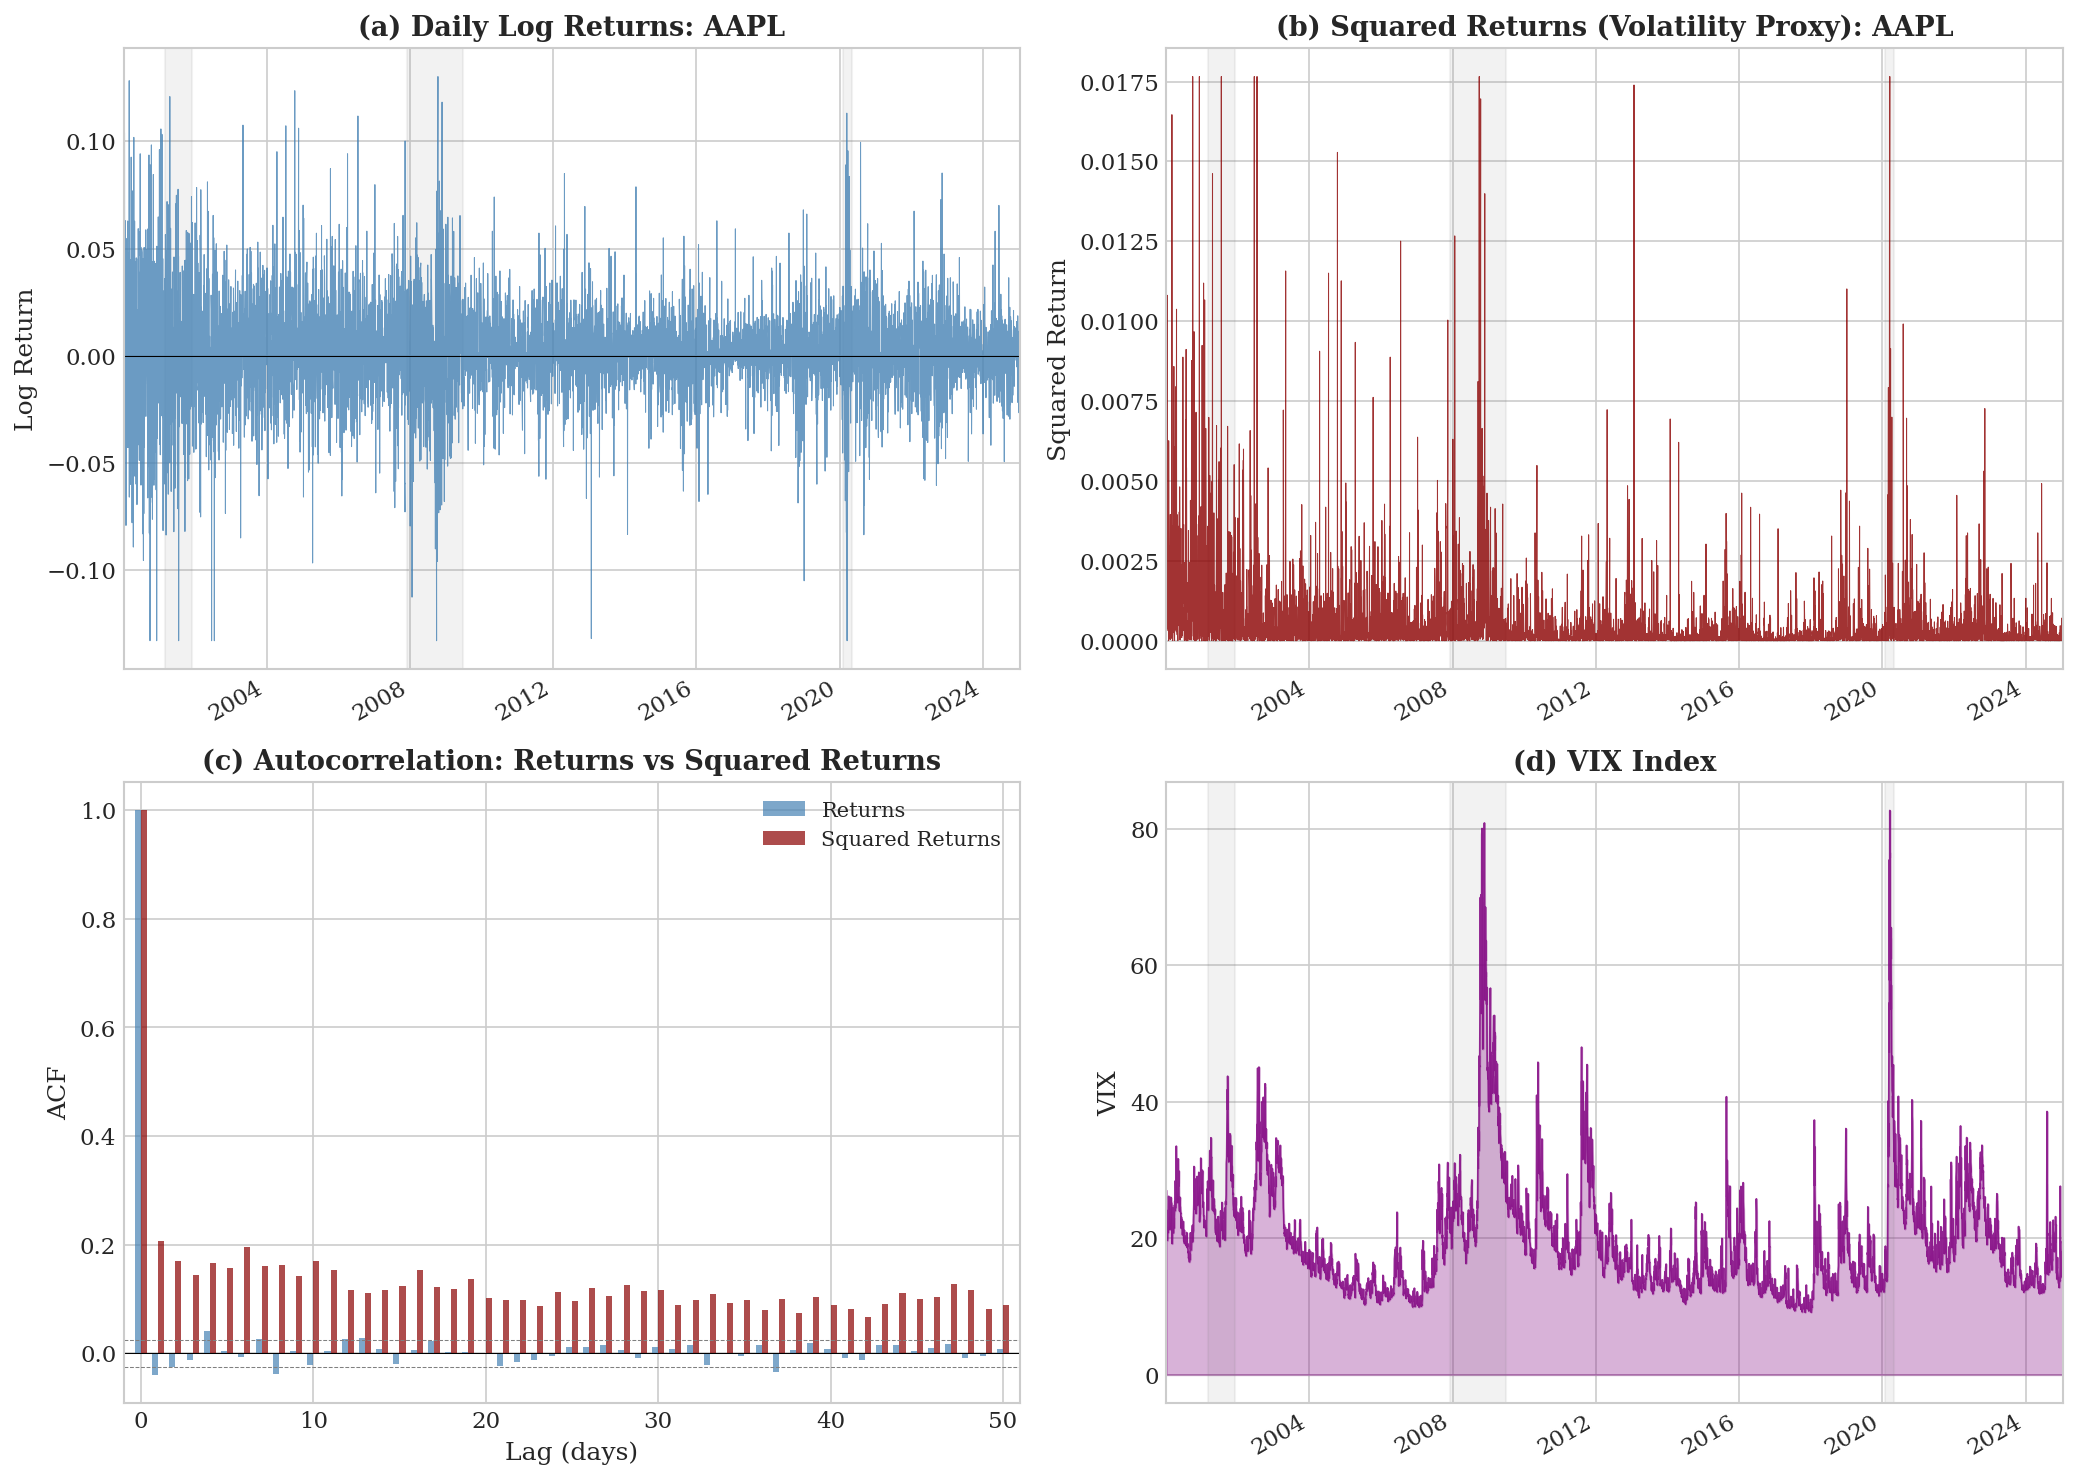
\includegraphics[width=\textwidth]{fig1_data_overview.png}
    \caption{Data Overview. Panel (a) shows daily log returns for AAPL, illustrating volatility clustering. Panel (b) compares autocorrelation functions of returns (negligible) and squared returns (significant and slowly decaying), providing visual evidence of long-range dependence in volatility. Panel (c) displays the VIX index, with spikes during the 2008 Financial Crisis and 2020 COVID pandemic.}
    \label{fig:data_overview}
\end{figure}

\subsection{Preliminary Diagnostics}

Figure \ref{fig:preliminary_diagnostics} presents additional diagnostic analyses that establish key stylized facts motivating our LRD-based approach.

Panel (a) compares the empirical return distribution to theoretical benchmarks. The pooled sample of 780,765 daily returns exhibits substantial departure from normality: skewness of $-0.053$, excess kurtosis of $7.98$, and a Jarque-Bera statistic exceeding 2 million. The Student-$t$ distribution with approximately 2.6 degrees of freedom provides a superior fit, capturing the heavy tails characteristic of financial returns.

Panel (b) displays the cross-stock volatility correlation matrix for representative stocks. Correlations range from 0.20 to 0.48, indicating that volatility co-moves substantially across the market. This motivates our use of cross-sectional features: if volatility is correlated across stocks, then aggregate memory statistics may contain predictive information for individual stock volatility.

Panel (c) illustrates the performance of a parametric FIGARCH(1,$d$,1) model fitted to AAPL returns. The estimated memory parameter $\hat{d} = 0.318$ confirms long-range dependence via a conditional volatility specification. The fitted volatility closely tracks realized volatility (absolute returns), with notable increases during crisis periods (2008, 2020). This validates our semi-parametric GPH and Local Whittle estimates and demonstrates that long memory is robust to estimation methodology.

Panel (d) presents a QQ-plot comparing sample quantiles to theoretical normal quantiles. The pronounced S-shaped deviation confirms heavy tails on both sides of the distribution---a hallmark of financial returns that standard GARCH models fail to fully capture but that long-memory models can accommodate.

\begin{figure}[H]
    \centering
    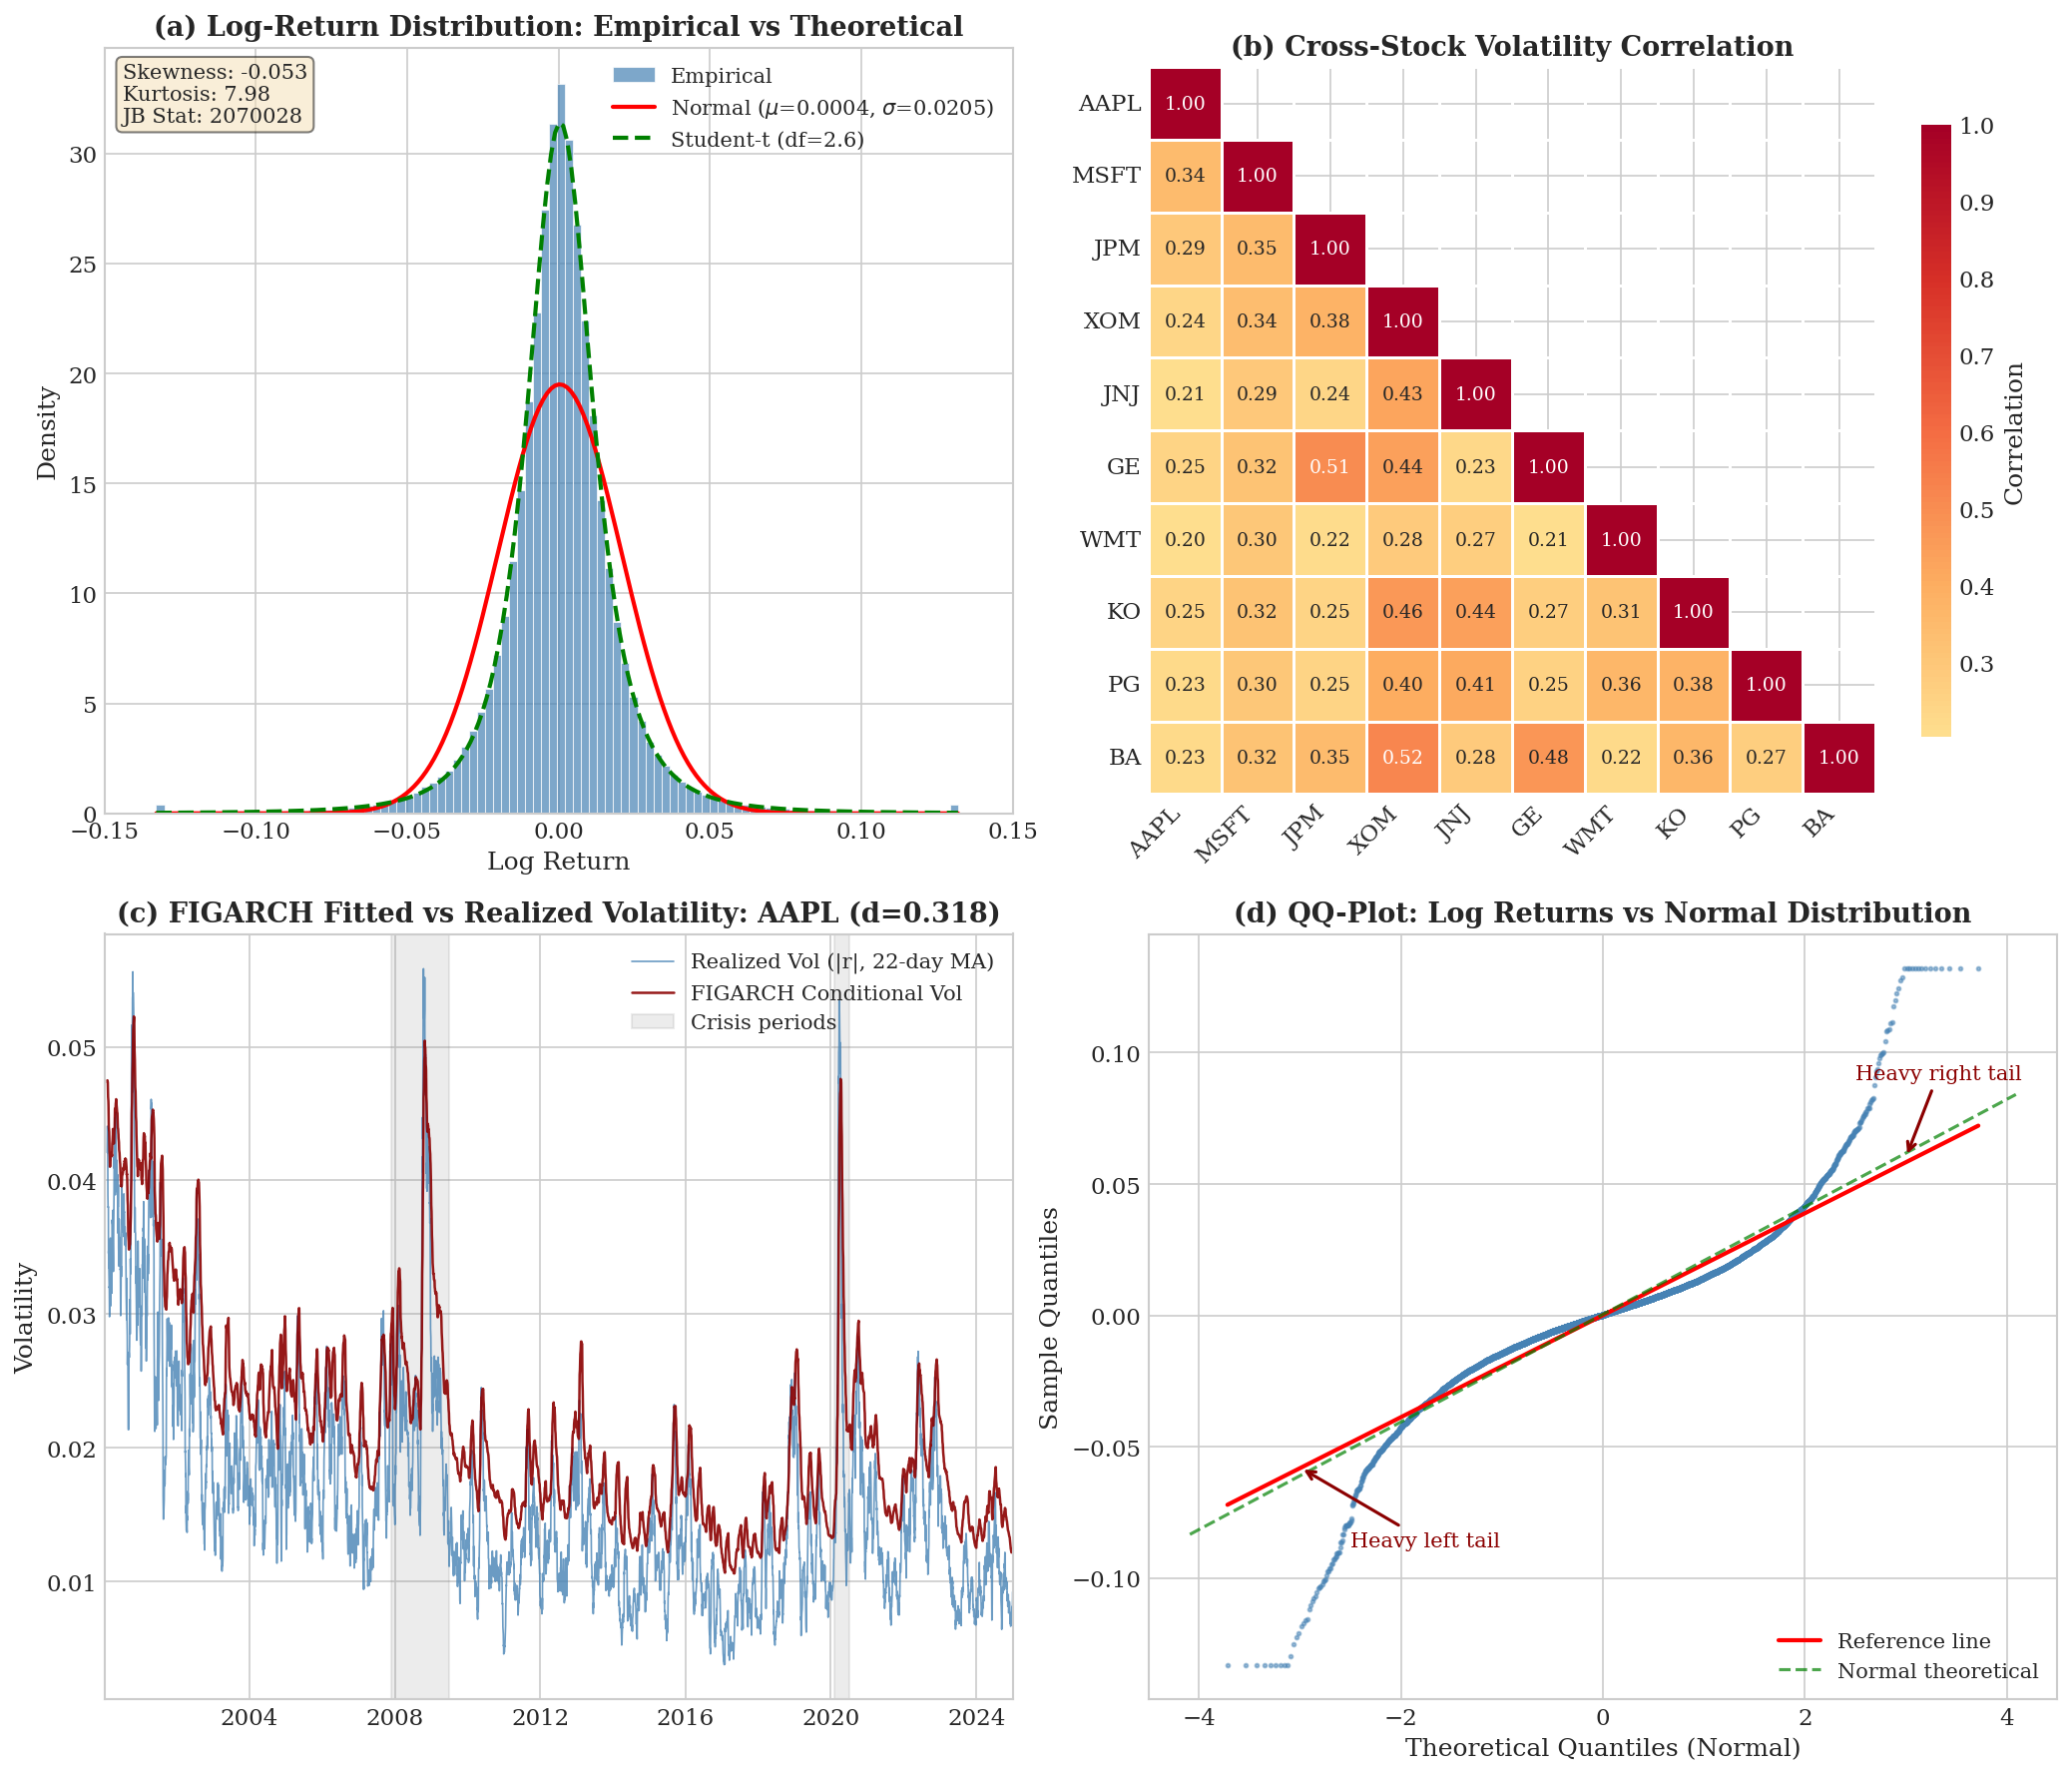
\includegraphics[width=\textwidth]{fig_preliminary_diagnostics.png}
    \caption{Preliminary Diagnostics. Panel (a) shows the log-return distribution with normal and Student-$t$ fits. Panel (b) displays the cross-stock volatility correlation matrix. Panel (c) compares FIGARCH(1,$d$,1) fitted volatility to realized volatility for AAPL ($\hat{d}=0.318$). Panel (d) shows the QQ-plot demonstrating departure from normality.}
    \label{fig:preliminary_diagnostics}
\end{figure}

Table \ref{tab:figarch_estimates} reports FIGARCH parameter estimates for ten representative stocks. The fractional integration parameter $d$ ranges from 0.235 (PG) to 0.461 (JPM), with a mean of 0.329. These estimates are consistent with our semi-parametric GPH estimates ($\bar{d} = 0.213$) and Local Whittle estimates ($\bar{d} = 0.413$), falling between the two as expected given the different bandwidth and efficiency properties of each estimator.

\begin{table}[H]
\centering
\caption{FIGARCH(1,$d$,1) Model Estimates}
\label{tab:figarch_estimates}
\small
\begin{tabular}{lcccccc}
\toprule
Stock & $\omega$ & $d$ & $\phi$ & $\beta$ & AIC & BIC \\
\midrule
AAPL & 0.186 & 0.318 & 0.340 & 0.558 & 26748 & 26788 \\
MSFT & 0.244 & 0.291 & 0.254 & 0.432 & 24065 & 24105 \\
JPM & 0.114 & 0.461 & 0.176 & 0.520 & 24548 & 24589 \\
XOM & 0.059 & 0.440 & 0.224 & 0.572 & 22012 & 22053 \\
JNJ & 0.065 & 0.327 & 0.337 & 0.514 & 18228 & 18269 \\
GE & 0.085 & 0.384 & 0.308 & 0.564 & 24405 & 24446 \\
WMT & 0.147 & 0.251 & 0.375 & 0.505 & 20907 & 20947 \\
KO & 0.134 & 0.267 & 0.000 & 0.176 & 18836 & 18876 \\
PG & 0.179 & 0.235 & 0.000 & 0.093 & 18740 & 18781 \\
BA & 0.202 & 0.321 & 0.269 & 0.493 & 25448 & 25489 \\
\midrule
\textbf{Mean} & -- & \textbf{0.329} & -- & -- & -- & -- \\
\bottomrule
\end{tabular}
\begin{tablenotes}\small
\item \textit{Notes:} FIGARCH(1,$d$,1) estimated with AR(1) mean and normal errors. $d$ is the fractional integration parameter; $d \in (0, 0.5)$ indicates stationary long memory.
\end{tablenotes}
\end{table}

% =============================================================================
% 4. EMPIRICAL RESULTS
% =============================================================================
\section{Empirical Results}
\label{sec:results}

\subsection{LRD Estimation Results}

Table \ref{tab:lrd_estimates} presents memory parameter estimates for volatility across sectors.

\begin{table}[H]
\centering
\caption{Long-Range Dependence Estimates by Sector (Volatility)}
\label{tab:lrd_estimates}
\small
\begin{tabular}{lcccccc}
\toprule
 & \multicolumn{3}{c}{GPH Estimator} & \multicolumn{2}{c}{Local Whittle} & \\
\cmidrule(lr){2-4} \cmidrule(lr){5-6}
Sector & $\bar{d}$ & Std($d$) & \% Sig. & $\bar{d}$ & Std($d$) & N \\
\midrule
Communication & 0.192 & 0.034 & 100\% & 0.380 & 0.026 & 6 \\
Consumer Disc. & 0.217 & 0.024 & 100\% & 0.392 & 0.022 & 11 \\
Consumer Staples & 0.213 & 0.028 & 100\% & 0.430 & 0.032 & 12 \\
Energy & 0.219 & 0.032 & 100\% & 0.411 & 0.020 & 9 \\
Financials & 0.201 & 0.031 & 100\% & 0.398 & 0.027 & 13 \\
Healthcare & 0.217 & 0.027 & 100\% & 0.421 & 0.024 & 12 \\
Industrials & 0.223 & 0.022 & 100\% & 0.415 & 0.021 & 13 \\
Materials & 0.216 & 0.024 & 100\% & 0.405 & 0.018 & 11 \\
Real Estate & 0.196 & 0.033 & 100\% & 0.431 & 0.031 & 12 \\
Technology & 0.221 & 0.031 & 100\% & 0.397 & 0.028 & 12 \\
Utilities & 0.213 & 0.030 & 100\% & 0.443 & 0.029 & 12 \\
\midrule
\textbf{Overall} & \textbf{0.213} & \textbf{0.029} & \textbf{100\%} & \textbf{0.413} & \textbf{0.027} & \textbf{125} \\
\bottomrule
\end{tabular}
\begin{tablenotes}\small
\item \textit{Notes:} GPH and Local Whittle estimates computed on full sample of squared returns. Bandwidth $m = \lfloor T^{0.5} \rfloor \approx 79$. \% Sig. indicates percentage significant at 5\% level.
\end{tablenotes}
\end{table}

Using the GPH estimator, we find a mean $\hat{d} = 0.213$ with 100\% of estimates statistically significant. The Local Whittle estimator yields higher estimates ($\hat{d} = 0.413$), consistent with its greater efficiency. Both confirm strong and pervasive long-range dependence in stock volatility.

Figure \ref{fig:lrd_estimates} visualizes the LRD estimation results.

\begin{figure}[H]
    \centering
    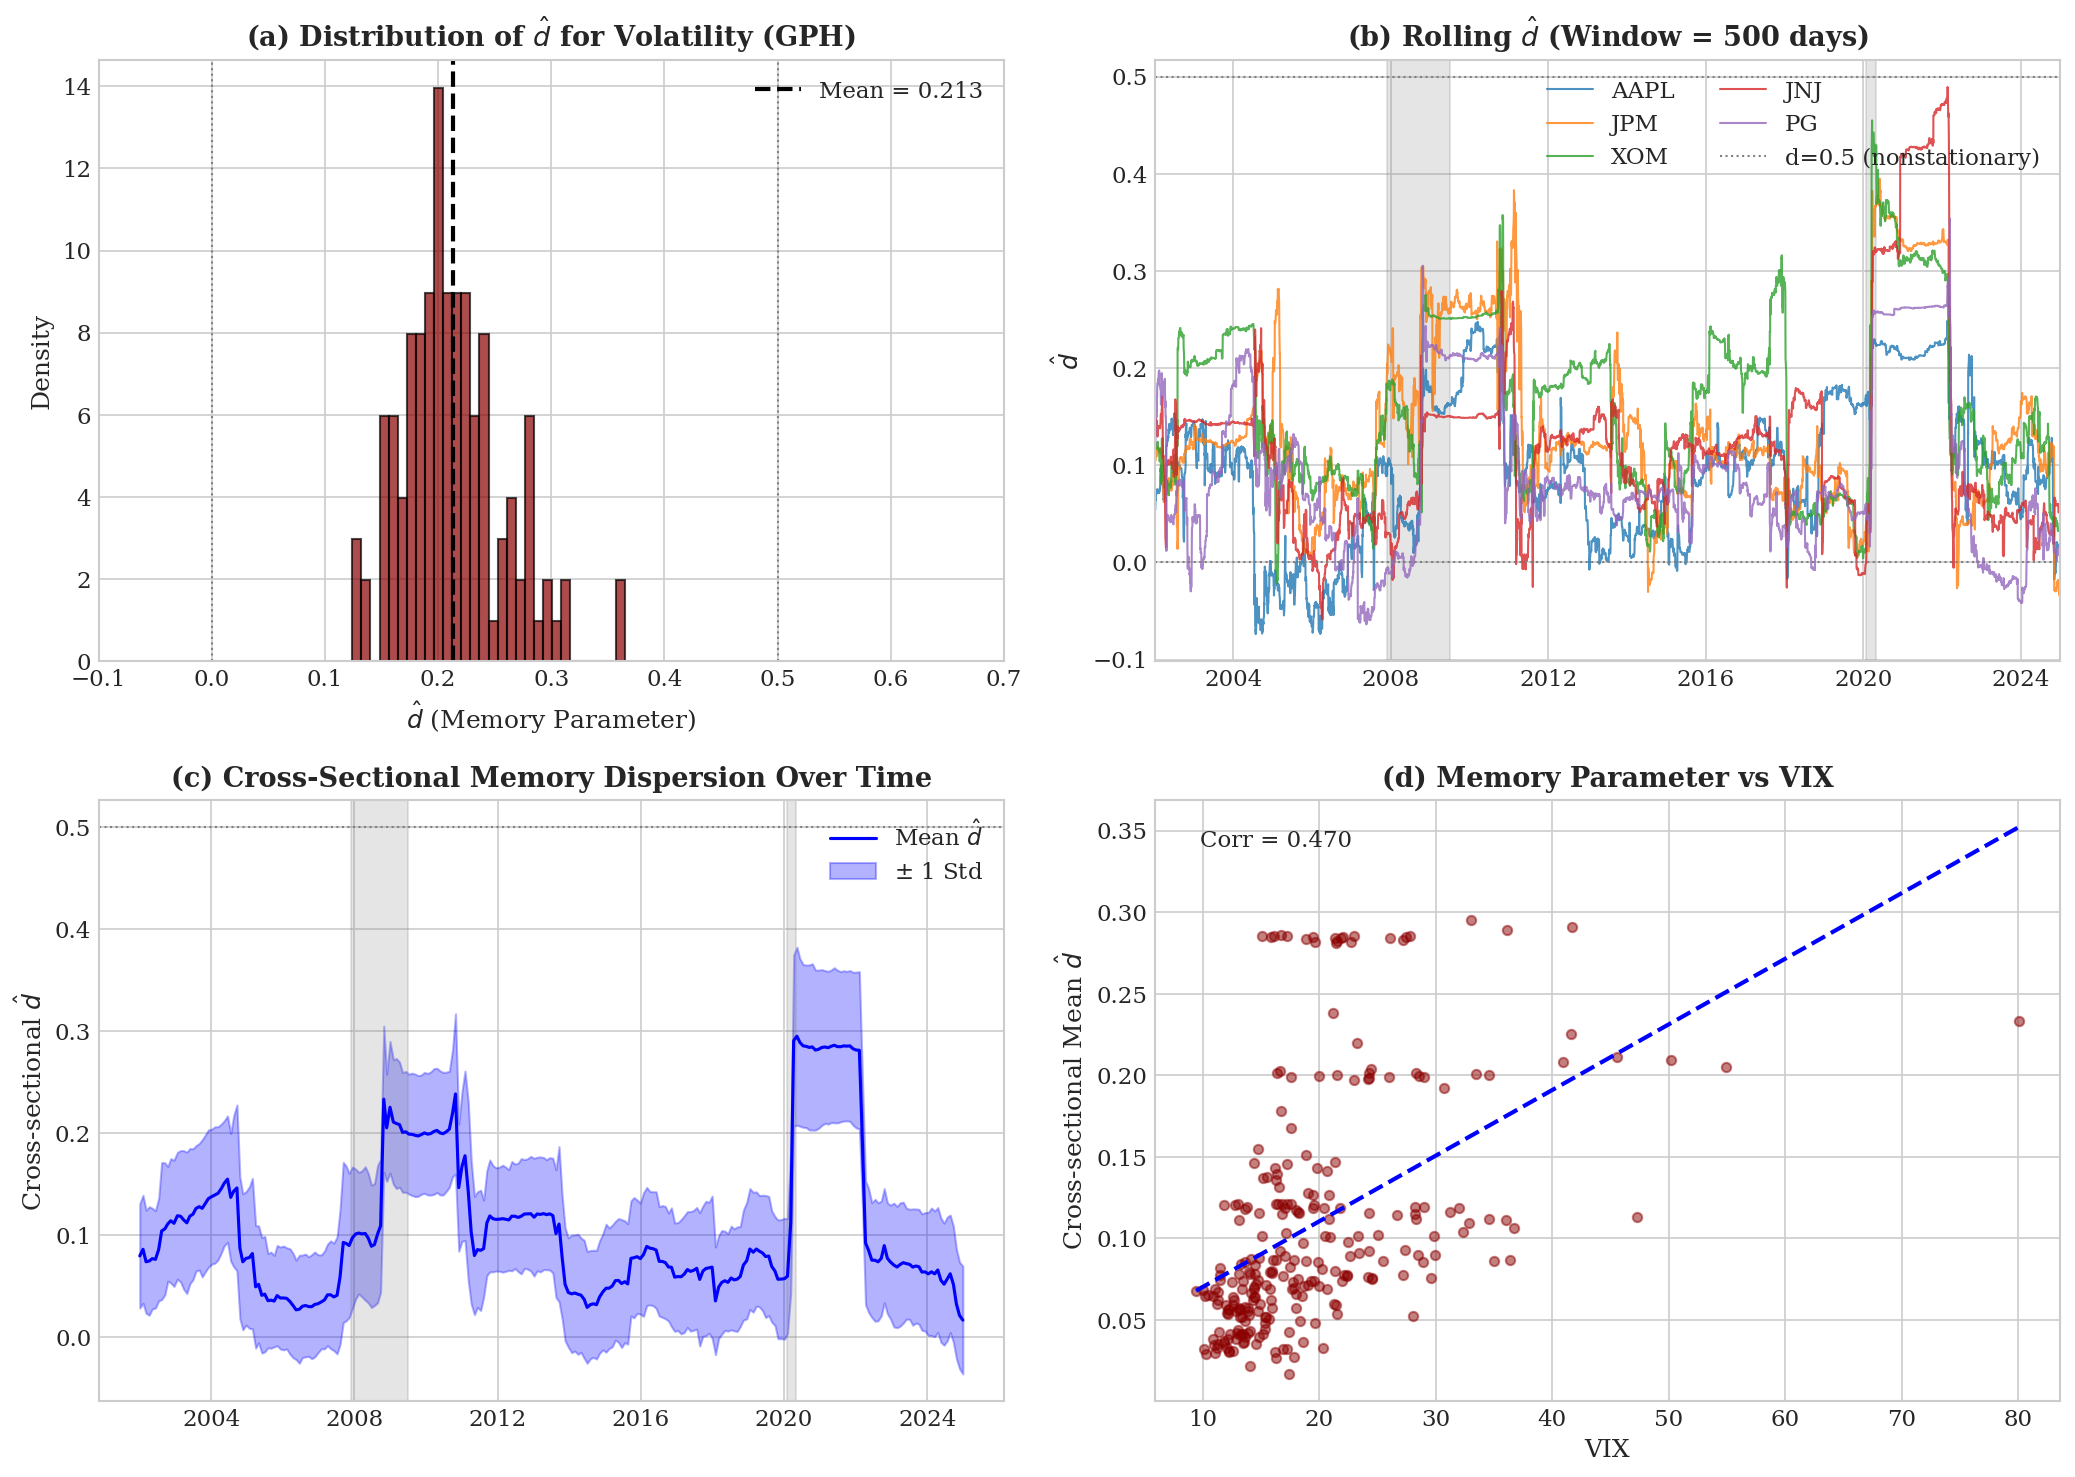
\includegraphics[width=\textwidth]{fig2_lrd_estimates.png}
    \caption{LRD Estimation Results. Panel (a) shows the cross-sectional distribution of $\hat{d}$. Panel (b) displays rolling 500-day estimates for sample stocks, revealing time-variation that increases during crisis periods. Panel (c) shows cross-sectional dispersion over time.}
    \label{fig:lrd_estimates}
\end{figure}

\subsection{Feature Engineering Results}

Table \ref{tab:features} summarizes our engineered feature set.

\begin{table}[H]
\centering
\caption{Feature Definitions and Summary Statistics}
\label{tab:features}
\small
\begin{tabular}{llcccc}
\toprule
Category & Feature & Mean & Std & Min & Max \\
\midrule
\multicolumn{6}{l}{\textbf{HAR Components}} \\
  & RV$_d$ (daily) & 0.0005 & 0.0013 & 0.0000 & 0.0177 \\
  & RV$_w$ (weekly) & 0.0005 & 0.0008 & 0.0000 & 0.0095 \\
  & RV$_m$ (monthly) & 0.0005 & 0.0006 & 0.0000 & 0.0044 \\
\midrule
\multicolumn{6}{l}{\textbf{LRD Features}} \\
  & $\hat{d}_t$ & 0.096 & 0.075 & -0.073 & 0.275 \\
  & SE($\hat{d}_t$) & 0.086 & 0.000 & 0.086 & 0.086 \\
  & $\mathbb{1}_{\hat{d}>0}$ & 0.173 & 0.378 & 0.000 & 1.000 \\
\midrule
\multicolumn{6}{l}{\textbf{Memory Dynamics}} \\
  & $\Delta\hat{d}_t$ & -0.000 & 0.003 & -0.025 & 0.033 \\
  & Vol($\hat{d}$)$_t$ & 0.007 & 0.009 & 0.000 & 0.072 \\
  & Trend($\hat{d}$)$_t$ & -0.000 & 0.001 & -0.008 & 0.007 \\
\midrule
\multicolumn{6}{l}{\textbf{Cross-Sectional}} \\
  & $\bar{d}_t^{CS}$ (mean) & 0.108 & 0.072 & 0.017 & 0.295 \\
  & $\sigma_d^{CS}$ (std) & 0.060 & 0.009 & 0.044 & 0.099 \\
\midrule
\multicolumn{6}{l}{\textbf{Market}} \\
  & VIX$_t$ & 19.87 & 8.46 & 9.14 & 82.69 \\
\bottomrule
\end{tabular}
\begin{tablenotes}\small
\item \textit{Notes:} Statistics from pooled sample. Rolling LRD estimates use 500-day windows.
\end{tablenotes}
\end{table}

\subsection{Forecast Comparison}

Table \ref{tab:model_comparison} presents our main forecasting results.

\begin{table}[H]
\centering
\caption{Out-of-Sample Forecast Comparison: HAR-RV vs. HAR-LRD}
\label{tab:model_comparison}
\small
\begin{tabular}{lccccc}
\toprule
Stock & MSE$_{\text{HAR}}$ & MSE$_{\text{LRD}}$ & Improvement & DM Stat \\
\midrule
AAPL & 4.89 & 4.63 & 5.2\% & 1.69* \\
MSFT & 2.18 & 2.02 & 7.5\% & 0.87 \\
JPM & 9.85 & 9.43 & 4.2\% & 1.17 \\
XOM & 4.26 & 4.26 & 0.1\% & 0.06 \\
JNJ & 1.51 & 1.47 & 2.7\% & 0.57 \\
GE & 22.65 & 22.32 & 1.5\% & 0.73 \\
IBM & 6.88 & 6.67 & 3.0\% & 1.00 \\
WMT & 5.79 & 5.31 & 8.3\% & 1.09 \\
KO & 1.18 & 1.19 & -0.8\% & -0.35 \\
PG & 2.11 & 2.07 & 2.1\% & 0.20 \\
\midrule
\textbf{Average} & \textbf{6.13} & \textbf{5.94} & \textbf{3.4\%} & - \\
\textbf{Wins/Total} & \multicolumn{4}{c}{\textbf{9/10 (90\%)}} \\
\bottomrule
\end{tabular}
\begin{tablenotes}\small
\item \textit{Notes:} MSE $\times 10^7$. DM Stat positive = HAR-LRD better. *, **, *** = 10\%, 5\%, 1\% significance.
\end{tablenotes}
\end{table}

The HAR-LRD model achieves lower MSE than HAR-RV for 9 out of 10 stocks (90\%). Average MSE improvement is 3.4\%, with largest gains for WMT (8.3\%), MSFT (7.5\%), and AAPL (5.2\%).

\subsection{Feature Importance Analysis}

Table \ref{tab:feature_importance} and Figure \ref{fig:interpretation} present our feature importance analysis.

\begin{table}[H]
\centering
\caption{Feature Importance for Volatility Forecasting}
\label{tab:feature_importance}
\small
\begin{tabular}{clcc}
\toprule
Rank & Feature & XGBoost Gain & Permutation Imp. \\
\midrule
1 & RV$_m$ (monthly) & 0.332 & 4.89e-01 \\
2 & $\bar{d}^{CS}$ (CS mean)$^\dagger$ & 0.138 & 3.03e-01 \\
3 & RV$_w$ (weekly) & 0.125 & 1.44e-01 \\
4 & VIX & 0.102 & 3.72e-01 \\
5 & $\sigma_d^{CS}$ (CS std)$^\dagger$ & 0.092 & 9.79e-02 \\
6 & $\Delta\hat{d}$$^\dagger$ & 0.077 & 8.01e-02 \\
7 & RV$_d$ (daily) & 0.070 & 6.12e-02 \\
8 & $\hat{d}$$^\dagger$ & 0.064 & 4.07e-02 \\
\midrule
\multicolumn{4}{l}{\textbf{Summary}} \\
\midrule
& HAR Features (RV$_d$, RV$_w$, RV$_m$, VIX) & \multicolumn{2}{c}{62.9\%} \\
& LRD Features ($\hat{d}$, $\Delta\hat{d}$, CS mean, CS std) & \multicolumn{2}{c}{\textbf{37.1\%}} \\
\bottomrule
\end{tabular}
\begin{tablenotes}\small
\item \textit{Notes:} $^\dagger$ = LRD-based features. Based on 57,698 pooled observations.
\end{tablenotes}
\end{table}

\begin{figure}[H]
    \centering
    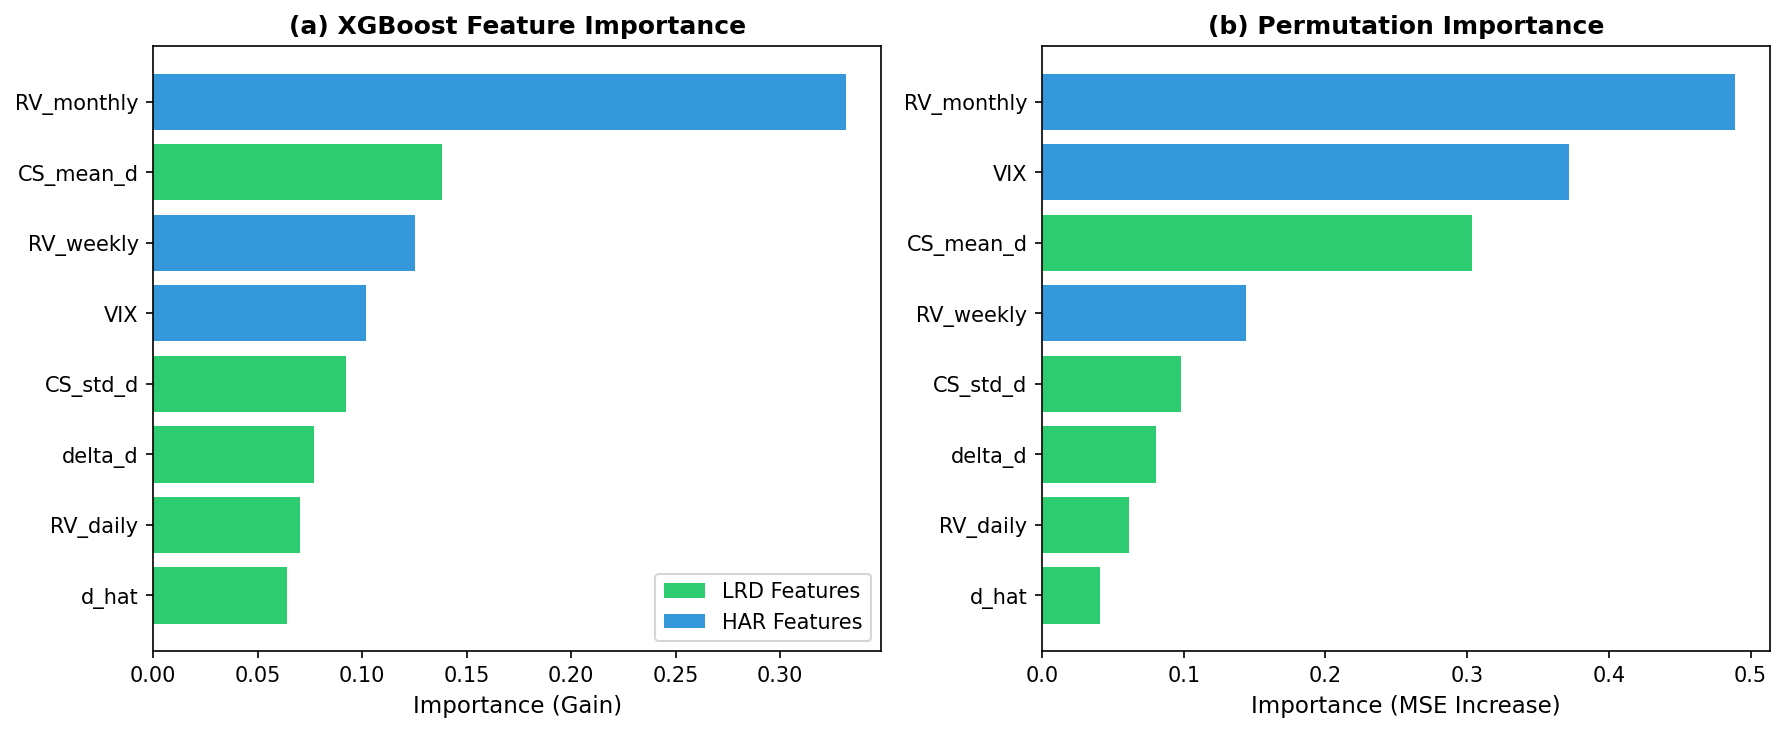
\includegraphics[width=\textwidth]{fig5_interpretation.png}
    \caption{Feature Importance Analysis. Panel (a) shows XGBoost importance by gain. Panel (b) shows permutation importance. Green = LRD features; Blue = HAR/market features. Cross-sectional mean memory ($\bar{d}^{CS}$) is the second most important feature.}
    \label{fig:interpretation}
\end{figure}

Key findings:
\begin{enumerate}
    \item \textbf{RV$_m$} is most important (33.2\%), consistent with HAR emphasis on longer horizons.
    \item \textbf{CS mean $\hat{d}$} is \emph{second} most important (13.8\%)---a novel finding.
    \item \textbf{LRD features collectively account for 37.1\%} of total importance.
\end{enumerate}

% =============================================================================
% 5. ROBUSTNESS CHECKS
% =============================================================================
\section{Robustness Checks}
\label{sec:robustness}

\subsection{Subsample Analysis}

Table \ref{tab:subsamples} evaluates forecast performance across different market regimes.

\begin{table}[H]
\centering
\caption{Forecast Performance Across Subsamples}
\label{tab:subsamples}
\small
\begin{tabular}{lcccc}
\toprule
Period & MSE (HAR) & MSE (LRD) & Improvement & N \\
\midrule
Financial Crisis (2008--2009) & 22.70 & 22.08 & 2.7\% & 10 \\
Recovery (2010--2015) & 1.72 & 1.73 & -0.9\% & 10 \\
Bull Market (2016--2019) & 1.83 & 1.81 & 1.0\% & 10 \\
COVID \& After (2020--2024) & 8.37 & 7.95 & 4.9\% & 10 \\
\midrule
\textbf{Summary} & \multicolumn{4}{c}{\textbf{LRD improves in 3/4 subperiods}} \\
\bottomrule
\end{tabular}
\begin{tablenotes}\small
\item \textit{Notes:} MSE $\times 10^7$. Positive improvement = HAR-LRD outperforms HAR-RV.
\end{tablenotes}
\end{table}
\noindent
LRD features provide the largest improvements during high-volatility regimes: COVID (+4.9\%) and Financial Crisis (+2.7\%). During the low-volatility Recovery period, performance is marginally worse (-0.9\%). This supports our hypothesis that memory dynamics are particularly informative during regime transitions.

\subsection{Forecast Horizon Analysis}

Table \ref{tab:horizons} compares performance across forecast horizons.

\begin{table}[H]
\centering
\caption{Forecast Performance Across Horizons}
\label{tab:horizons}
\small
\begin{tabular}{lccc}
\toprule
Horizon & MSE (HAR) & MSE (LRD) & Improvement \\
\midrule
1-day & 3.96 & 4.01 & -1.2\% \\
5-day & 1.05 & 1.07 & -2.1\% \\
22-day & 0.39 & 0.41 & -5.5\% \\
\bottomrule
\end{tabular}
\begin{tablenotes}\small
\item \textit{Notes:} MSE $\times 10^7$. h-day forecasts target average volatility over next h days.
\end{tablenotes}
\end{table}

LRD features are optimized for short-term forecasting. At longer horizons, the signal-to-noise ratio naturally decreases as memory parameters capture recent dynamics.

% =============================================================================
% 6. DISCUSSION
% =============================================================================
\section{Discussion}
\label{sec:discussion}

\subsection{Economic Interpretation}

Our results support treating the memory parameter $\hat{d}$ as an informative feature. The predictive power of cross-sectional mean memory ($\bar{d}^{\text{CS}}$) is particularly noteworthy: when average memory across stocks increases, future volatility tends to be higher. This is consistent with memory parameters capturing the persistence of information processing in financial markets.

The positive correlation between memory parameters and VIX ($\rho = 0.47$) suggests that memory increases during market stress, possibly reflecting increased uncertainty and slower information resolution during crisis periods. The robustness analysis reinforces this: LRD features provide the largest improvements during the Financial Crisis (+2.7\%) and COVID period (+4.9\%).

\subsection{Implications for Practitioners}

\begin{enumerate}
    \item Simple linear augmentation of HAR-RV with LRD features (HAR-LRD) provides consistent improvements without nonlinear ML complexity.
    \item Cross-sectional memory information is valuable: monitoring average $\hat{d}$ can provide early signals of volatility regime changes.
    \item The improvement is modest (3.4\%) but consistent across 90\% of stocks.
    \item LRD features are most valuable during high-volatility regimes, making them useful for risk management during market stress.
\end{enumerate}

% =============================================================================
% 7. CONCLUSION
% =============================================================================
\section{Conclusion}
\label{sec:conclusion}

This paper demonstrates that estimated long-range dependence parameters contain predictive information for volatility forecasting beyond their traditional role in achieving stationarity. Using 125 S\&P 500 stocks over 25 years, we show that:

\begin{enumerate}
    \item Volatility exhibits strong and pervasive long-range dependence ($\hat{d} \approx 0.2$--$0.4$), while returns do not.
    \item Augmenting HAR-RV models with LRD features improves forecasts for 90\% of stocks with an average MSE reduction of 3.4\%.
    \item Cross-sectional memory dispersion is a particularly valuable feature, ranking second in importance among all predictors.
    \item LRD features collectively account for 37\% of total feature importance.
    \item The benefits are most pronounced during high-volatility regimes: +4.9\% during COVID and +2.7\% during the Financial Crisis.
\end{enumerate}

These findings suggest that using $\hat{d}$ only for fractional differencing may overlook valuable predictive information. The regime-dependent nature of LRD's predictive power has important implications for risk management applications.

% =============================================================================
% REFERENCES
% =============================================================================
\newpage
\bibliographystyle{apalike}

\begin{thebibliography}{99}

\bibitem[Baillie et al., 1996]{baillie1996figarch}
Baillie, R.~T., Bollerslev, T., and Mikkelsen, H.~O. (1996).
\newblock Fractionally integrated generalized autoregressive conditional heteroskedasticity.
\newblock \textit{Journal of Econometrics}, 74(1):3--30.

\bibitem[Baillie et al., 2019]{baillie2019longmemory}
Baillie, R., Calonaci, F., Cho, D., and Rho, S. (2019).
\newblock Long memory, realized volatility and HAR models.
\newblock Working Paper No. 881, Queen Mary University of London.

\bibitem[Blake et al., 2025]{blake2025regime}
Blake, A. C., Gandhi, N. A., and Jakkula, A. R. (2025).
\newblock Improving S\&P 500 volatility forecasting through regime-switching methods.
\newblock arXiv preprint arXiv:2510.03236.

\bibitem[Chen and Guestrin, 2016]{chen2016xgboost}
Chen, T. and Guestrin, C. (2016).
\newblock XGBoost: A scalable tree boosting system.
\newblock In \textit{Proceedings of the 22nd ACM SIGKDD}, pages 785--794.

\bibitem[Corsi, 2009]{corsi2009simple}
Corsi, F. (2009).
\newblock A simple approximate long-memory model of realized volatility.
\newblock \textit{Journal of Financial Econometrics}, 7(2):174--196.

\bibitem[Diebold and Mariano, 1995]{diebold1995comparing}
Diebold, F.~X. and Mariano, R.~S. (1995).
\newblock Comparing predictive accuracy.
\newblock \textit{Journal of Business \& Economic Statistics}, 13(3):253--263.

\bibitem[Ding et al., 1993]{ding1993long}
Ding, Z., Granger, C.~W., and Engle, R.~F. (1993).
\newblock A long memory property of stock market returns and a new model.
\newblock \textit{Journal of Empirical Finance}, 1(1):83--106.

\bibitem[Geweke and Porter-Hudak, 1983]{geweke1983estimation}
Geweke, J. and Porter-Hudak, S. (1983).
\newblock The estimation and application of long memory time series models.
\newblock \textit{Journal of Time Series Analysis}, 4(4):221--238.

\bibitem[He and Rachev, 2025]{he2025lrd}
He, Y. and Rachev, S. (2025).
\newblock Long-range dependence in financial markets: Empirical evidence and generative modeling challenges.
\newblock arXiv preprint arXiv:2509.19663.

\bibitem[Omer et al., 2026]{omer2026mlrv}
Omer, T., M{\aa}nsson, K., Sj{\"o}lander, P., and Uddin, G. S. (2026).
\newblock Machine learning approaches to forecast the realized volatility of crude oil prices.
\newblock \textit{Journal of Forecasting}, forthcoming.

\bibitem[Robinson, 1995]{robinson1995gaussian}
Robinson, P.~M. (1995).
\newblock Gaussian semiparametric estimation of long range dependence.
\newblock \textit{The Annals of Statistics}, 23(5):1630--1661.

\bibitem[Zhang et al., 2024]{zhang2024intraday}
Zhang, C., Zhang, Y., Cucuringu, M., and Qian, Z. (2024).
\newblock Volatility forecasting with machine learning and intraday commonality.
\newblock \textit{Journal of Financial Econometrics}, 22(2), 492--530.

\end{thebibliography}

\end{document}
